\section{OpenNMS Community}
In \emph{OpenNMS} there is a global community consisting of developers, corporations, service providers, researchers and users. The following section will give you a short overview which main roles exist in the community.

\subsection*{Role of \emph{The OpenNMS Group}}
The software OpenNMS is provided under the free license GPLv3+. What is the reason for a commercial company behind it? The company \emph{The OpenNMS Group, Inc.} provides professional support and gives people a place who want to spend significant time of their life to the project. Code development in commercial environment is reflected as a code contribution to the free software project. \emph{The OpenNMS Group, Inc.} provides the following publicly available infrastructure:

\begin{itemize}
  \item Continous integration to build, test, compile and deploy OpenNMS.
  \item Packaging and providing infrastructure distributing pre-compiled packages for different operating systems and \emph{Linux/Unix} distributions
  \item Issue tracking for bugs, enhancements and feature requests
  \item Providing and running mailing lists
  \item Maintaining the software branches and source code repository
  \item Organizing and plan the software release management
\end{itemize}

\subsection*{Order of the Green Polo}
The super secret brotherhood (OGP) and developers of the \emph{OpenNMS Project}. You can recognize and \emph{OGP} member by their good looks as well as their super-flashy, very coveted \emph{OpenNMS Green Polo}. As Tarus Balog said:
 
\begin{quote}
Back in fall of 2004, I wanted to find a way to recognize those people who make \emph{OpenNMS} what it is, and to thank them in some fashion. 
Ever since the advent of "business casual" workplace attire, the "logo" polo shirt has become a fixture in IT departments around the world. We sell black and white polos with the \emph{OpenNMS} logo on our web site.

But this is much, much, much, different. These are "green" polos, very rare, and they will never be available for sale. Think of them as equivalent to winning \emph{The Masters} golf tournament's green jacket - only harder to get.
In order to get one, all one has to do is give up all hope of having a life outside of \emph{OpenNMS}, work long hours for free, and basically become a closed superhero, squashing bugs (or uncovering existence) in a single bound.
\end{quote}

\subsection*{OpenNMS Foundation Europe}
To cover non-commercial interests the \emph{OpenNMS Foundation Europe e.V.} (OFE) was founded in July 31st. in Fulda, Germany. It is a registered non-profit organization in Germany. 

The objective of the organization is to promote the use, develop, educate and research around free software and network (management) technologies, especially \emph{OpenNMS}. To do this, the \emph{OFE} organizes conferences and trainings and acts as an advocate for free open source software. The \emph{OFE} initiates software development and studies which are made available to the public under the \emph{GPL}\footnote{GNU General Public License: \url{http://www.gnu.org/licenses/gpl.html}} or a suitable successor.

\subsection*{Your Contribution to OpenNMS}
There are many ways to become a part of the project. Most of our more experienced users run through the \emph{DFLTC} (duffel-td) lifecycle.
\begin{itemize}
  \item \textit{\textbf{D}download} the software and start to get familiar with it 
  \item \textit{\textbf{F}ail} and try make your first steps on the learning curve
  \item \textit{\textbf{L}earn} the use of OpenNMS with others or with content they provide in Blogs or Wiki pages.
  \item \textit{\textbf{T}rain} people and help them to improve their knowledge about OpenNMS and network mangement
  \item \textit{\textbf{C}contribute} with your gained knowledge to improve the project and the community
\end{itemize}
If you are a user or developer, there are many ways to contribute a free software project. As users you can help to improve documentation, spend configuration or help others in IRC, mailing list or by local beerings\footnote{Your funny note here}.

If you are a developer and you would like contribute source code to OpenNMS, you have to sign the \emph{OpenNMS Contributor Agreement}. It allows \textit{The OpenNMS Group, Inc.} to publish your code contribution under GPLv3+. You can find the agreement at the following link \url{http://www.opennms.org/wiki/Contributor_Agreement}. 

\subsection*{Where is the code}
The source code is hosted on \emph{GitHub}\footnote{\url{http://www.github.com}}. 



Code contributions can be merged into \emph{OpenNMS} with \emph{pull requests}. The workflow to get your source code into \emph{OpenNMS} is shown in picture \ref{fig:contrib-workflow} on page \pageref{fig:contrib-workflow}.
\begin{figure}
	\centering
	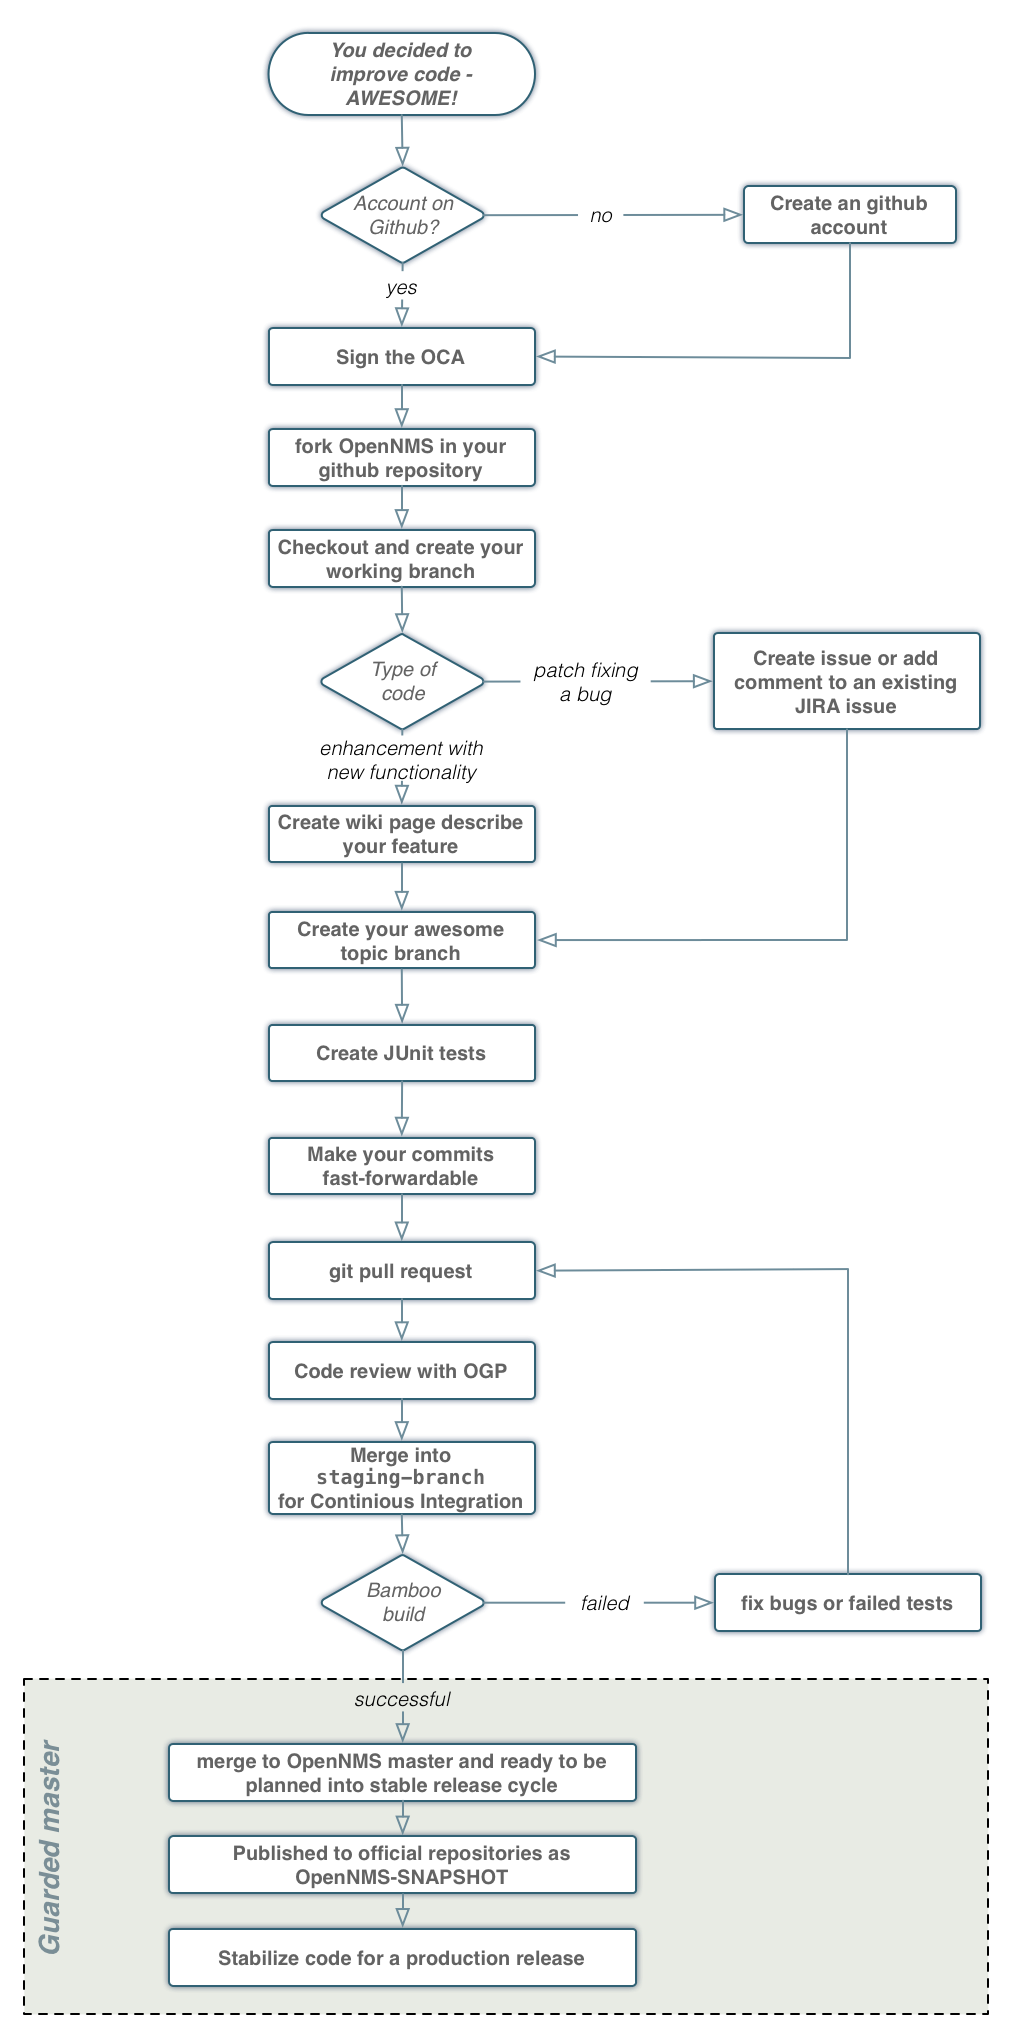
\includegraphics[width=0.75\textwidth]{images/contribution-workflow.png}
	\caption{Workflow for code contribution}
	\label{fig:contrib-workflow}
\end{figure}

\subsection*{Get your IDE up and running}
The \emph{OpenNMS} project is written in \emph{Java}. To maintain and handle external libraries it uses \emph{Maven}. It contains even more advanced technologies like \emph{OSGi} for class loading and \emph{Vaadin} as user interface framework. As version control system the project uses \emph{git}. To get an introduction working with \emph{git} and get your development environment up and running you can find documentation on the following wiki pages:
\begin{itemize}
  \item \url{http://www.opennms.org/wiki/Developing_with_Git}
  \item \url{http://www.opennms.org/wiki/Eclipse_and_OpenNMS}
\end{itemize}

\subsection*{Issue tracking, code browser and build system}
To document bugs, enhancements and feature request, the \emph{OpenNMS Group, Inc.} provide and maintains a public \emph{Atlassian JIRA} installation. It is recommended you create your JIRA account, which allows you to document bugs, enhancements or feature requests. The application for issue and feature tracking is available on \url{http://issues.opennms.org}.

The \emph{OpenNMS} software development follows a test driven approach. To provide a stable and continous quality of the code base, the \emph{OpenNMS Group} provides and run \emph{Atlassian Bamboo} as a build system. It compiles, tests and deploys the \emph{OpenNMS} software from the public \emph{git} repositories. The build system is public available on \url{http://bamboo.internal.opennms.com:8085}.

\emph{The OpenNMS Group} provides public access to \emph{Atlassian Fisheye} which gives the possibility to browse code from a browser and search for commit messages. The code browser is available on \url{http://fisheye.opennms.org}.